%
%  Name: Delayed Bisimulation
%  For: obsidian notes
%  Created: 2025-10-03
%
\documentclass{standalone}
\usepackage{amsmath}
\usepackage{tikz}
\usetikzlibrary{arrows,automata,positioning}

\usepackage{xcolor}
\definecolor{halcyon-base-blue-01}{HTML}{171c28}    % Workbench Background
\definecolor{halcyon-base-blue-01}{HTML}{1d2433}    % Editor Background
\definecolor{halcyon-base-blue-03}{HTML}{2f3b54}    % Highlight, widgets, panel
\definecolor{halcyon-base-blue-04}{HTML}{6679a4}    % Dividers, subtle UI elements
\definecolor{halcyon-base-blue-05}{HTML}{8695b7}    % Status bar text, buttons, etc.
\definecolor{halcyon-base-grey-dark}{HTML}{a2aabc}  % Variables, property names, tabs
\definecolor{halcyon-base-grey-light}{HTML}{d7dce2} % Active text, anything that should be white

\definecolor{halcyon-accent}{HTML}{ffcc66}          % Accent, list tree titles, badges, etc.

\definecolor{halcyon-palette-cyan}{HTML}{5ccfe6}    % - UI: Modified highlights
\definecolor{halcyon-palette-lime}{HTML}{bae67e}    % - UI: Addition highlights
\definecolor{halcyon-palette-orange}{HTML}{ffae57}  % Constants, operators
\definecolor{halcyon-palette-yellow}{HTML}{ffd580}  % Functions, classes, object literal keys
\definecolor{halcyon-palette-lilac}{HTML}{c3a6ff}   % Keywords, constants, template literals
\definecolor{halcyon-palette-salmon}{HTML}{ef6b73}  % Deletion highlights, errors, warnings

\begin{document}

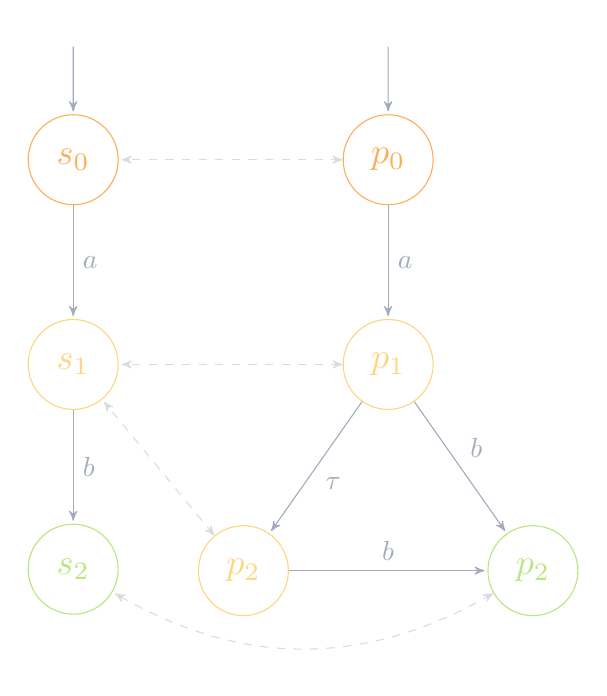
\begin{tikzpicture}[>=stealth', shorten >=1pt,node distance=2cm,auto]
  \tikzstyle{every state}=[style={scale=1.3}]

  %% L1
  \node                                (l1)                           {};
  \node[state, halcyon-palette-orange] (s0) [below of=l1, yshift=8mm] {$s_0$};
  \node[state, halcyon-palette-yellow] (s1) [below of=s0]             {$s_1$};
  \node[state, halcyon-palette-lime]   (s2) [below of=s1]             {$s_2$};

  %% Spacing
  \node (space) [right of=l1] {};

  %% L2
  \node                                (l2) [right of=space]                {};
  \node[state, halcyon-palette-orange] (p0) [below of=l2, yshift=8mm]       {$p_0$};
  \node[state, halcyon-palette-yellow] (p1) [below of=p0]                   {$p_1$};
  \node[state, halcyon-palette-yellow] (p2) [below left of=p1, yshift=-6mm] {$p_2$};
  \node[state, halcyon-palette-lime]   (p3) [below right of=p1,yshift=-6mm] {$p_2$};
  
  %% L1 path
  \path[->,halcyon-base-grey-dark]
    (l1) edge node {}    (s0)
	  (s0) edge node {$a$} (s1)
	  (s1) edge node {$b$} (s2);
  
  %% L2 path
  \path[->,halcyon-base-grey-dark]
	  (l2) edge node {}       (p0)
	  (p0) edge node {$a$}    (p1)
	  (p1) edge node {$\tau$} (p2)
	  (p1) edge node {$b$}    (p3)
	  (p2) edge node {$b$}    (p3);
  
  %% Bisim arrows
  \path[dashed,<->,halcyon-base-grey-light] 
	  (p0) edge node {} (s0)
	  (p1) edge node {} (s1)
	  (p2) edge node {} (s1);
  \path[dashed, <->, halcyon-base-grey-light]
	  (p3) edge[bend left] node {} (s2);
\end{tikzpicture}

\end{document}